\documentclass[12pt]{article}
\usepackage[a4paper,margin=1in]{geometry}
\usepackage{amsmath, amssymb}
\usepackage{graphicx}
\usepackage{booktabs}
\usepackage{hyperref}
\usepackage{algorithm}
\usepackage{algorithmic}
\usepackage{caption}
\usepackage{natbib}

\title{An Integer Programming Approach to Solving Rummikub Configurations}
\author{Your Name \\ Department of Computer Science \\ Your University}
\date{\today}

\begin{document}

\sloppy
\maketitle

\begin{abstract}
\sloppy
Rummikub is a popular tile-based game that involves both combinatorial optimization and strategic decision-making. This paper presents a formal investigation into the game mechanics, identifies the core computational challenges, and introduces an integer programming (IP) model designed to find optimal moves for a given player state. We analyze the problem space, define constraints based on legal game rules, and propose an IP formulation to maximize score per turn. Computational experiments validate the model’s effectiveness and provide insights into its potential for AI agent development.
\end{abstract}

\section{Introduction}
Rummikub is a classic tile-laying game blending elements of rummy and mahjong. Its complexity arises from its dynamic board, flexible tile arrangements, and constraint-based rules. While humans rely on heuristics, we aim to explore a formal mathematical model that can generate optimal plays automatically.

\subsection{Motivation}
Understanding the strategic depth of Rummikub can aid in creating intelligent agents for game-playing and provide case studies in integer programming applications.

\section{Background and Related Work}
\subsection{Rummikub Game Rules Overview}
Each player starts with 14 tiles. The goal is to create valid sets (groups or runs) to reduce one's hand to zero. A group is three or four tiles of the same number in different colors. A run is three or more consecutive numbers of the same color.

\subsection{Computational Complexity}
Previous research suggests that determining a valid move is NP-hard due to the permutations and combinations of tile arrangements.~\cite{rummikub_complexity}.


\subsection{Related AI Models}
Discuss existing models or papers on game AI, such as those used in Sudoku, Scrabble, or other combinatorial games.

\section{Integer Programming Model}
\subsection{Problem Definition}
Given a hand of tiles and the current board state, determine the optimal move (or series of moves) that maximizes score.

\subsection{Model Assumptions}
\begin{itemize}
    \item All tiles and their colors are encoded numerically.
    \item The board is flattened to a list of valid sets.
    \item Initial meld rules and joker rules are incorporated.
\end{itemize}

\subsection{Variables and Parameters}
Let $x_{ijk}$ be a binary variable indicating if tile $i$ is used in group/run $j$ in position $k$.

Define:
\begin{itemize}
    \item $T$: set of all tiles
    \item $G$: set of possible groups/runs
    \item $B$: board state
    \item $H$: hand tiles
\end{itemize}

\subsection{Constraints}
\begin{itemize}
    \item Each tile used only once per turn
    \item Groups/runs must follow valid Rummikub rules
    \item At least 30 points for the initial meld (if first move)
\end{itemize}

\subsection{Objective Function}
\[
\max \sum_{i \in H} \sum_{j \in G} \sum_{k} v_i \cdot x_{ijk}
\]
where $v_i$ is the value of tile $i$ (equal to its number).

\section{Implementation and Experiments}
\subsection{Tools Used}
Model implemented using Python and solved with Google OR-Tools / Gurobi / CPLEX.

\subsection{Test Cases}
Present example game states and corresponding optimal plays derived from the model.

\begin{figure}[h]
    \centering
    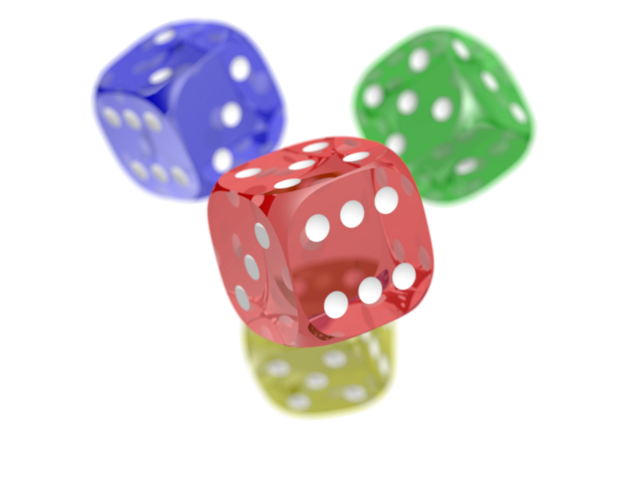
\includegraphics[width=0.7\textwidth]{Figures/example_image.png}
    \caption{Example board configuration solved by the model.}
\end{figure}

\subsection{Results}
Show performance in terms of solution time, move quality, and comparison with heuristic approaches.

\section{Discussion}
\subsection{Limitations}
\begin{itemize}
    \item Model scalability as board complexity increases
    \item Handling dynamic player interaction
\end{itemize}

\subsection{Future Work}
\begin{itemize}
    \item Integration with other AI agents.
    \item Use of reinforcement learning or hybrid approaches.
\end{itemize}

\section{Conclusion}
We have proposed an integer programming model capable of identifying optimal Rummikub moves from a static game state. This framework serves as a step toward developing intelligent agents capable of playing competitively.

\bibliographystyle{plainnat}
\bibliography{rummikub_research}

\end{document}
